\section{Úvod do problematiky}
Saliency a teda detekcia významných oblastí je využívaná rôznych oblastiach. Počínajúc automatizáciou je tažiskom pri segmentácií obrazu alebo detekcíi špecifických objektov. Od saliency modelov sú taktiež závyslé aj programy ovládajúce zabezpečovacie zariadenia. Až po reklamu kde je vyzuálna pozornosť klúčovým parametrom čo može rozhodnúť o úspechu produktu, veď aký význam by mala reklama kde si nevšimnete prezentovaný produkt, alebo si všimnete iba jeho "menej" dokonalé časti.
\section{Metody pre statické obrázky}
Algoritmy pre statické obrazy tvoria základ všetkých saliency modelov a tvoria najstaršiu oblasť výskumu. V tejto časti uvediem prehľad algoritmov pre výpočet saliency modelov od najjednoduchších cez najznámejšie až po nejefektívnejšie. Na záver uvediem porovnanie všetkých metód pomocou všeobecne uznávaných metrík a dát získaných z zariadní merajúcich pohyb očí používateľa (eyetrackera).
\subsection{Baseline Center}\label{section:caseline-center}
Baseline center je triviálny model ktorý sa vypočítava pomocou Gaussovej krivky vzľadom na pomer strán čím predpokladá salientné oblasti presne v strede obrazu. Nezachytáva však žiadne sémantické aspekty videa ako ani podvedome informácie vnímanania obrazu iba rozlíšenie dané optikou skenujúcou scénu.
TODO jeden obrazok-povodny/mapa/eyetracker vizualizacia
\subsection{Hrany}
Skupina algoritmov využívajúca význačné prechody v obraze inak nazývane hrany.
TODO
\subsection{Ittiho model}
Najznámejším modelom pre výpočet významných oblastí pre statické farebné obrazy je ittiho model navrhnutý v roku 1998. Model zakladá na rozložení obrazu na 3 základné charakteristiky obrazu a to farbu, intensitu, orientaciu.

\begin{wrapfigure}{r}{6cm}
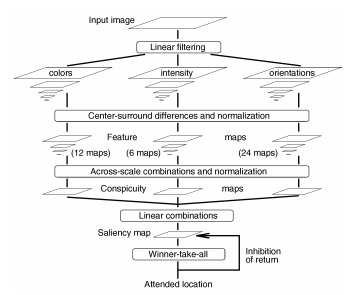
\includegraphics[width=7cm]{pics/itti-1.png}
\caption{Itti model general workflow.}\label{wrap-fig:1}
\end{wrapfigure}

Chrakteristika farby obsahuje 12 máp (šedotónové obrazy), pričom model používa farebný model RGB. Nazačiatku sa vypočíta intenzita podľa vztahu \begin{math} I = (R+G+B)/3\end{math}. Pomocou mapy I sa následne normalizujú všetky farebné kanáli modelu RGB. Model extrahuje 4 farebné kanáli červený (r), zelený (g), modrý (b), zltý (y) a pomocou Gausvých pyramíd vytvorí 3 rôzne mapy každej farebnej zložky separátne. Červená zložka sa počíta difenčným spôsobom ako \begin{math} R = r - (g + b)/2 \end{math}, zelená ako \begin{math} G = g - (r + b)/2 \end{math}, modrá ako \begin{math}B = b - (r + g)/2\end{math} a žltá ako \begin{math}Y = (r + g)/2 - |r - g|/2 - b\end{math}. Chrakteristika intenzity obsahuje 6 máp. Získaná je pomocou orientovaných gáborových filtrov s orientáciou 0\degree, 45\degree, 90\degree, 135\degree. Dokopy 42 máp charakteristík je následne linárne skombinovaných do jednej saliency mapy\cite{itty-98}.


\subsection{Spektralne rezidua}
Medtóda využíva princím, že potláča štatisticky často opakujúce sa časti obrazu a do popredia stavia časti obrazu ktoré sa štatisticky odlišujú od ostatných. Na detekciu používa rýchlu fourierovu transformáciu. Pomocou nej rozdelí obrázok na amplitúdovú čast a fázovú čast. Amplitúdová zložka sa následne vyhladí čím sa do popredia dostanú iba informácie ktoré sa vymykajú z priemeru. Odčítaním od pôvodnej amplitúdoje zložky dostaneme iba časti obrazu ktoré sú významné \cite{spectral-rezidual}
TODO obrazok asi porovnanie s itty
\subsection{Sun Model}
\subsection{Rare Model}
...Context-Aware saliency, Weighted Maximum Phase Alignment Model, Torralba saliency, Murray model,
\section{Metody pre videá}
Video obsahuje rozsiahlejšie možnosti ako iba obrazová informácia, pribúdajú dalšie rozmery ako je pohyb objektov na obraze alebo vplyv zvuku na ľudské vnímanie. Avšak oproti obrazu obsahuje je potrebné spracovávať vedšie množtvo
dát. Navyše vo vedšine algoritmov využívajúcich saliency modely je potrebné aby model dával výsledky v reálnom čase. Používané hlavne v oblasti zabezpečovacej techniky.
\subsection{Zohladnenie audio informácie}
Saliency modely využívaju rôznorodé druhy príznakov a to od geneticky zakorenených ako sú prechody farieb, alebo intenzít, až po sémantické príznaky ako je detekcia tváre \cite{salient-faces}. Majoritná vedšina saliency modelov využíva iba obrazovú zložku ale zvuková stopa býva ponechaná stranou ale úplne zanedbaná. Použitie zvuku je známimtrikom filmovej scény uz desatročia, kde režiséri posilnujú kontrolu nad diváckou pozornosťou pomocou práve pomocou zvukového doporovodu. Prvé štúdie sa zaoberali detekciou reči a tváre, kde je spojitosť jednoznačná \cite{sound-1}. Neskoršie štúdie dokazujú korelácie aj na všeobecnejšej úrovni a pokusy o extrakciu samotnej charakteristiky zo zvukovej stopy\cite{sound-coutrot-1}. Tieto pokusy viedli aj zostaveniu modelov zohladnujúch zvukovú stopu ako samostatnú charakteristiku spolu s kombináciou s nízko-urovnovým príznami obrazu \cite{sound-courot-2}.

\begin{wrapfigure}{r}{5.5cm}
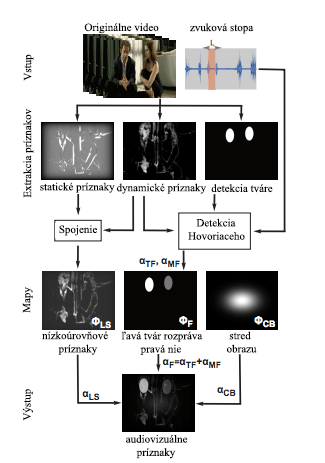
\includegraphics[width=7cm]{pics/courot-1.png}
\caption{Audiovisual model workflow.\cite{sound-courot-2}}\label{wrap-fig:1}
\end{wrapfigure}

Model extrahuje video na sekvenciu obrazov (framy) a audio stopu v tvare grafu vlnovej dĺžky. Potom extrahuje 3 typy rôznych chrakteristík. Nízko-úrovnové príznaky založené na biologicky inširovaných saliency modeloch rozdelených na dynamickú časť a satickú časť. Statická časť sa zameriava na najasnejšie a najkontrastnejšie časti obrazu. Dynamická časť sa zameriava na relatívny pohyb objektov vhľadom na pozadie (eliminácia pohybu kamery). Tieto 2 časti sa nakoniec spoja
Dalšou chrakteritikou použitou v tomto modeli je detekcia tváre. Každý objekt klasifikovaný ako tvár je v saliency mape nahradený oválnym objektom, intensita daných objetov je daná pomocou metódy Speaker Diarization, ktorá detekuje podľa zvukovej stopy objekt ktorý generuje zvuk. Metóda predpokladá striedavú konverzáciu n objektov oddelenú pauzou. Následne spojí vyššie spomýnané charakteristiky do jden výslednej mapy. Ako posledný krok preloží cez celú mapu baseline center model popísaný v časti \ref{section:caseline-center}.

\subsection{Detekcia pohybu}
V tejto časti sa zmeriame na segmentáciu objektov ktoré sa na scéne pohybujú. Taktéto obrazy sú v ľudskom vyzuálnom systéme vysoko hodnotené. Dôvody, prečo takto ludský vyzuálny systém pridáva prijoritu práve takýmto oblastiam možeme nájsť v antropológií (najsť zdroj!). Vysvetlenie je jednoduché a to snaha zabezpečit bezpečné prostredie okolo seba a všetko pohybujúce sa narušuje pocit bezpečnosti. V nasledujúcom texte rozoberieme 2 najpožívanejšie algoritmy používané na detekciu oblastí pohybu v obraze. Prvým z nich bude LUCAS KANADE[anotacia!], a druhým Horn Schunck[anotacia!].
TODO:
\iffalse
  #http://ieeexplore.ieee.org/xpl/login.jsp?tp=&arnumber=4269999&url=http%3A%2F%2Fieeexplore.ieee.org%2Fxpls%2Fabs_all.jsp%3Farnumber%3D4269999
\fi
\section{Metódy Využívajúce neurónové siete}
\section{Metriky úspešnosti}
Zobrat z MIT saliency
\section{Refenčné datasety}
RSD, SAVAM, AUDITORY DATASET
\section{Porovnanie štandardných Metód}
